\section{FP4 Contracts and Numerical Method}

\subsection{Related work}

Low-precision training builds on mixed-precision accumulation and stochastic
rounding \cite{gupta2015limited,micikevicius2018mixedprecision}. Early 4-bit
systems combined integer weights and activations with specialized gradient
formats \cite{sun2020ultralow}. Chmiel et al.'s logarithmic unbiased
quantization (LUQ) targets unbiased neural-gradient quantization over the full
range: it combines stochastic underflow below the smallest nonzero value,
range selection that avoids upper clipping, and stochastic rounding within a
logarithmic FP4 grid \cite{chmiel2023accurate}. This is a stronger construction
than applying ordinary adjacent-bin SR only inside the representable range.
FP8 and microscaling then established floating-point formats with shared block exponents
\cite{micikevicius2022fp8,rouhani2023microexponents,
rouhani2023microscaling,ocp2023mx}. Their behavior depends on more than bit
width: scale format, block geometry, tensor statistics, and the contraction
being quantized all matter
\cite{yang2025microscaling,hu2025designspace,sun2025scaling,fasoli2026finer}.

Recent FP4 pretraining systems make different choices along those axes. Tseng
et al. apply MXFP4 to the two backward matrix multiplications and combine
stochastic rounding with randomized Hadamard transform (RHT) preconditioning
\cite{tseng2025mxfp4}. FP4 All the Way uses round-to-nearest in Fprop and SR in
the backward and update contractions; in Wgrad, it stochastically rounds both
the neural-gradient and activation operands \cite{chmiel2025fp4alltheway}.
NVIDIA's NVFP4 recipe combines two-dimensional weights, gradient stochastic
rounding, paired Wgrad preconditioning, and selected higher-precision linears
\cite{nvidia2025nvfp4}. Quartet and FP4 All the Way study fully low-precision
paths, while subsequent work develops native
full-pipeline MXFP4 and unbiased NVFP4 gradient estimation
\cite{castro2025quartet,chmiel2025fp4alltheway,cim2026nativemxfp4,
panferov2026quartetii}.
Other FP4 studies examine optimizer and oscillation effects, adaptive block
scales, outlier dynamics, shrinkage bias, and quantization beyond the linear
operators
\cite{wang2025fp4,zhou2025exploringfp4,chen2025tetrajet,
chen2025tetrajetv2,cook2025fouroversix,dong2026outliers,
zhao2026ufp4,ding2026fullstack,agrusa2026whatmatters}. Complementary systems
explore spectral-domain FP4, alternative four-bit formats, and native FP4
training for mixture-of-experts models
\cite{cao2026metis,taghian2026hifloat4,du2026halfs,zhang2026hoppermoe}.
UE5M3 FP4 reallocates the unused sign bit of an E4M3 block scale to a fifth
exponent bit. Hu et al. combine this wider unsigned scale with periodic
sample-and-hold tensor scaling and selective backward SR, while omitting RHT
and using FP4 in every eligible internal linear
\cite{hu2026ue5m3}.

Three established mechanisms directly shape this work. A weight encoding can
remain numerically consistent under transposition
\cite{nvidia2025nvfp4,rahimifar2026transposition,cim2026nativemxfp4}.
Stochastic rounding can remove within-bin rounding bias, while its placement
and treatment of underflow and saturation remain part of the quantizer
contract \cite{gupta2015limited,chmiel2023accurate,ozkara2025sr}. Paired Hadamard preconditioning spreads
outliers while preserving the unquantized dot product
\cite{ashkboos2024quarot,tseng2025mxfp4,nvidia2025nvfp4,
cim2026nativemxfp4}. Our numerical contribution specializes where these
mechanisms act in each contraction and realizes that placement inside fused
training kernels.

The systems contribution is to optimize the quantizer, its physical layouts,
the consuming matrix multiplication, and retained backward state as one
execution boundary. This follows the broader principle that data movement and
producer--consumer structure determine realized model speed
\cite{dao2022flashattention,dao2023flashattention2,hsu2024liger,
wijmans2024cutcrossentropy,spector2024thunderkittens,guo2026coda}.

Table~\ref{tab:prior-work-boundary} pairs each established mechanism with the
concrete design delta implemented here.

\begin{table}[tbp]
  \centering
  \footnotesize
  \caption{Established numerical mechanisms and the concrete design delta
  implemented in this report.}
  \label{tab:prior-work-boundary}
  \begin{tabularx}{\textwidth}{@{}lYY@{}}
    \toprule
    Component & Established method & Our delta \\
    \midrule
    SR placement
      & Chmiel et al. use SR in Dgrad and on both Wgrad operands; NVIDIA applies
        gradient SR to both Dgrad and Wgrad
        \cite{chmiel2025fp4alltheway,nvidia2025nvfp4}
      & We apply SR only to the row-facing $dY$ consumed by Dgrad. Wgrad uses
        deterministic carriers, separating the two orientations of the same
        gradient tensor \\
    MXFP4 scale selection
      & E8M0 forces the block scale to a power of two. Rounding the exponent
        up keeps the block maximum within the finite E2M1 endpoint; rounding
        it down halves the decoded grid spacing while clamping the upper tail
        to that endpoint
        \cite{ocp2023mx,cim2026nativemxfp4}
      & We choose the scale policy by operand class. Development-only
        pretraining screens favored upward, encode-centric scales for
        activations and gradients; the 2D32 weight path admits the finer scale
        under a fixed tile-maximum test. The fused producer implements both
        rules \\
    2D weights
      & NVIDIA/TE use one 2D16 weight encoding across Fprop and Dgrad; 2D32
        transpose-consistent MXFP4 is also prior art
        \cite{nvidia2025nvfp4,nvidia2026te,rahimifar2026transposition,
        cim2026nativemxfp4}
      & Our fused 2D16 and 2D32 producers compute one orientation-consistent
        weight encoding and emit both physical consumer layouts when the scale
        domain completes \\
    Hadamard preconditioning
      & Tseng et al. randomize both MXFP4 backward GEMMs; NVIDIA uses one sampled
        sign vector throughout training for Wgrad; deterministic transforms are
        also prior art \cite{tseng2025mxfp4,nvidia2025nvfp4,cim2026nativemxfp4}
      & We make a fixed H16 or H32 sign diagonal part of the route contract,
        apply the same transform to $X$ and $dY$ for Wgrad only, and fuse it
        with column quantization \\
    Scale-aware fusion
      & NVFP4 uses a tensor-global outer scale, MXFP4 uses local power-of-two
        scales, and IO-aware fusion optimizes producer--consumer boundaries
        \cite{ocp2023mx,nvidia2025nvfp4,dao2022flashattention,guo2026coda}
      & Global v5 overlaps the tensor reduction; CTA-local NVFP4 carries two
        tile-owned outer factors; both co-produce layouts and saved state at the
        scale-completion boundary \\
    Hybrid assignment
      & Prior recipes vary precision by layer or module
        \cite{zhou2025exploringfp4,nvidia2025nvfp4,
        rahimifar2026transposition}
      & The operand hybrid assigns MXFP4 or CTA-local NVFP4 per contraction
        within every linear, motivated by a same-state Dgrad error analysis \\
    \bottomrule
  \end{tabularx}
\end{table}
\FloatBarrier

\subsection{The same four-bit values, three different scale contracts}
\label{sec:scale-contracts}

All three native routes ultimately present E2M1 operands---one sign bit, two
exponent bits, and one fraction bit---to a Blackwell Tensor Core. Their
numerical and scheduling behavior nevertheless
differs because they assign scales to different domains.  A useful common
notation for one scalar is
\begin{equation}
  \widehat z_i = S\,\delta_{b(i)}
  Q_{\mathrm{E2M1}}\!\left(\frac{z_i}{S\,\delta_{b(i)}}\right),
  \label{eq:hierarchical-quant}
\end{equation}
where $\delta_{b(i)}$ is the effective block dequantization multiplier, $S$
is an optional outer scale, and
$Q_{\mathrm{E2M1}}$ rounds and saturates to E2M1.  The scale choice determines
both quantization error and when the producer may safely release its output.

\begin{table}[tbp]
  \centering
  \caption{The FP4 execution contracts used in this report. CTA-local
  NVFP4 is an implementation policy, not a new datatype.}
  \label{tab:format-contracts}
  \begin{tabularx}{\textwidth}{lccY}
    \toprule
    Route & Block & Scale metadata & Main systems consequence \\
    \midrule
    \mxfp{} & 32 & E8M0 block scale & Local reduction; coarse power-of-two grid \\
    Global \nvfp{} v5 & 16 & E4M3 block + FP32 tensor & Requires the completed tensor amax \\
    \localcta{} & 16 & E4M3 block + two FP32 tile-outer scales & Tile-local production; two-sided metadata \\
    \bottomrule
  \end{tabularx}
\end{table}
\FloatBarrier

E8M0 represents a power-of-two scale with eight exponent bits and no fraction;
E4M3 is an FP8 scale with four exponent and three fraction bits. In \mxfp{},
$S=1$, $s_b$ is an E8M0 power of two shared by 32 values, and the effective
multiplier in Equation~\ref{eq:hierarchical-quant} is $\delta_b=s_b/6$.
The block maximum therefore produces a scale locally, but adjacent scale
levels differ by exactly two. This leaves a consequential choice about which
neighboring power of two to store.

We call upward exponent rounding \emph{encode-centric} scaling because it
first encloses every source value in a scale that E2M1 can encode without
upper-tail clipping. For a positive, finite block maximum
$a_b=\max_i|z_i|$ within the supported E8M0 exponent range, it computes
\begin{equation}
  s_b=2^{\lceil\log_2 a_b\rceil},\qquad
  q_i=Q_{\mathrm{E2M1}}\!\left(\frac{6z_i}{s_b}\right),\qquad
  \widehat z_i=\frac{s_b}{6}q_i.
  \label{eq:mxfp4-encode-scale}
\end{equation}
The largest magnitude then maps to at most the finite E2M1 endpoint, 6. We
call downward exponent rounding \emph{decode-centric} scaling: it chooses
$s_b=2^{\lfloor\log_2 a_b\rfloor}$ so the decoded multiplier $s_b/6$ is half
as large whenever $a_b$ is not already a power of two. That halves the grid
spacing for values that remain in range, but values above the endpoint
saturate to 6 and lose their excess magnitude. In plain terms,
encode-centric scaling protects the largest value; decode-centric scaling
represents smaller values more finely by accepting clipping at the top of the
block. For example, if $a_b=10$, encode-centric scaling stores $s_b=16$ and
does not clip; decode-centric scaling stores $s_b=8$, halves the spacing, and
clips values whose magnitude exceeds 8.

We expose this direction as part of the MXFP4 route rather than treating it as
an incidental implementation detail. Development-only MXFP4 pretraining
screens favored encode-centric over decode-centric scaling for both activation
and gradient operands. These screens selected the recipe; they are not a
reported quantitative comparison. All reported \mxfp{}-v4 routes therefore use
Equation~\ref{eq:mxfp4-encode-scale} for those operands.

Weights use a different trade-off. The orientation-consistent 2D32 producer
starts from the safe upward-rounded scale $s_T$ for the maximum $a_T$ over a
$32\!\times\!32$ tile. For a nonzero tile with a representable safe exponent,
it selects $s_T/2$ only when $a_T/s_T<0.87$. The smaller scale halves the
quantization spacing and accepts a fixed, bounded amount of upper-tail
clipping. The same fused producer makes that decision once and emits both
physical consumer layouts. Our MXFP4 contribution is this explicit
operand-dependent scale policy together with its fused implementation;
neither upward nor downward E8M0 rounding is a new number format.

E8M0 scale stochastic rounding is disabled in these recipes. ``Row-SR''
elsewhere in the paper instead denotes stochastic rounding of the E2M1
gradient payload; it does not randomize the E8M0 scale exponent.

\begin{figure}[tbp]
  \centering
  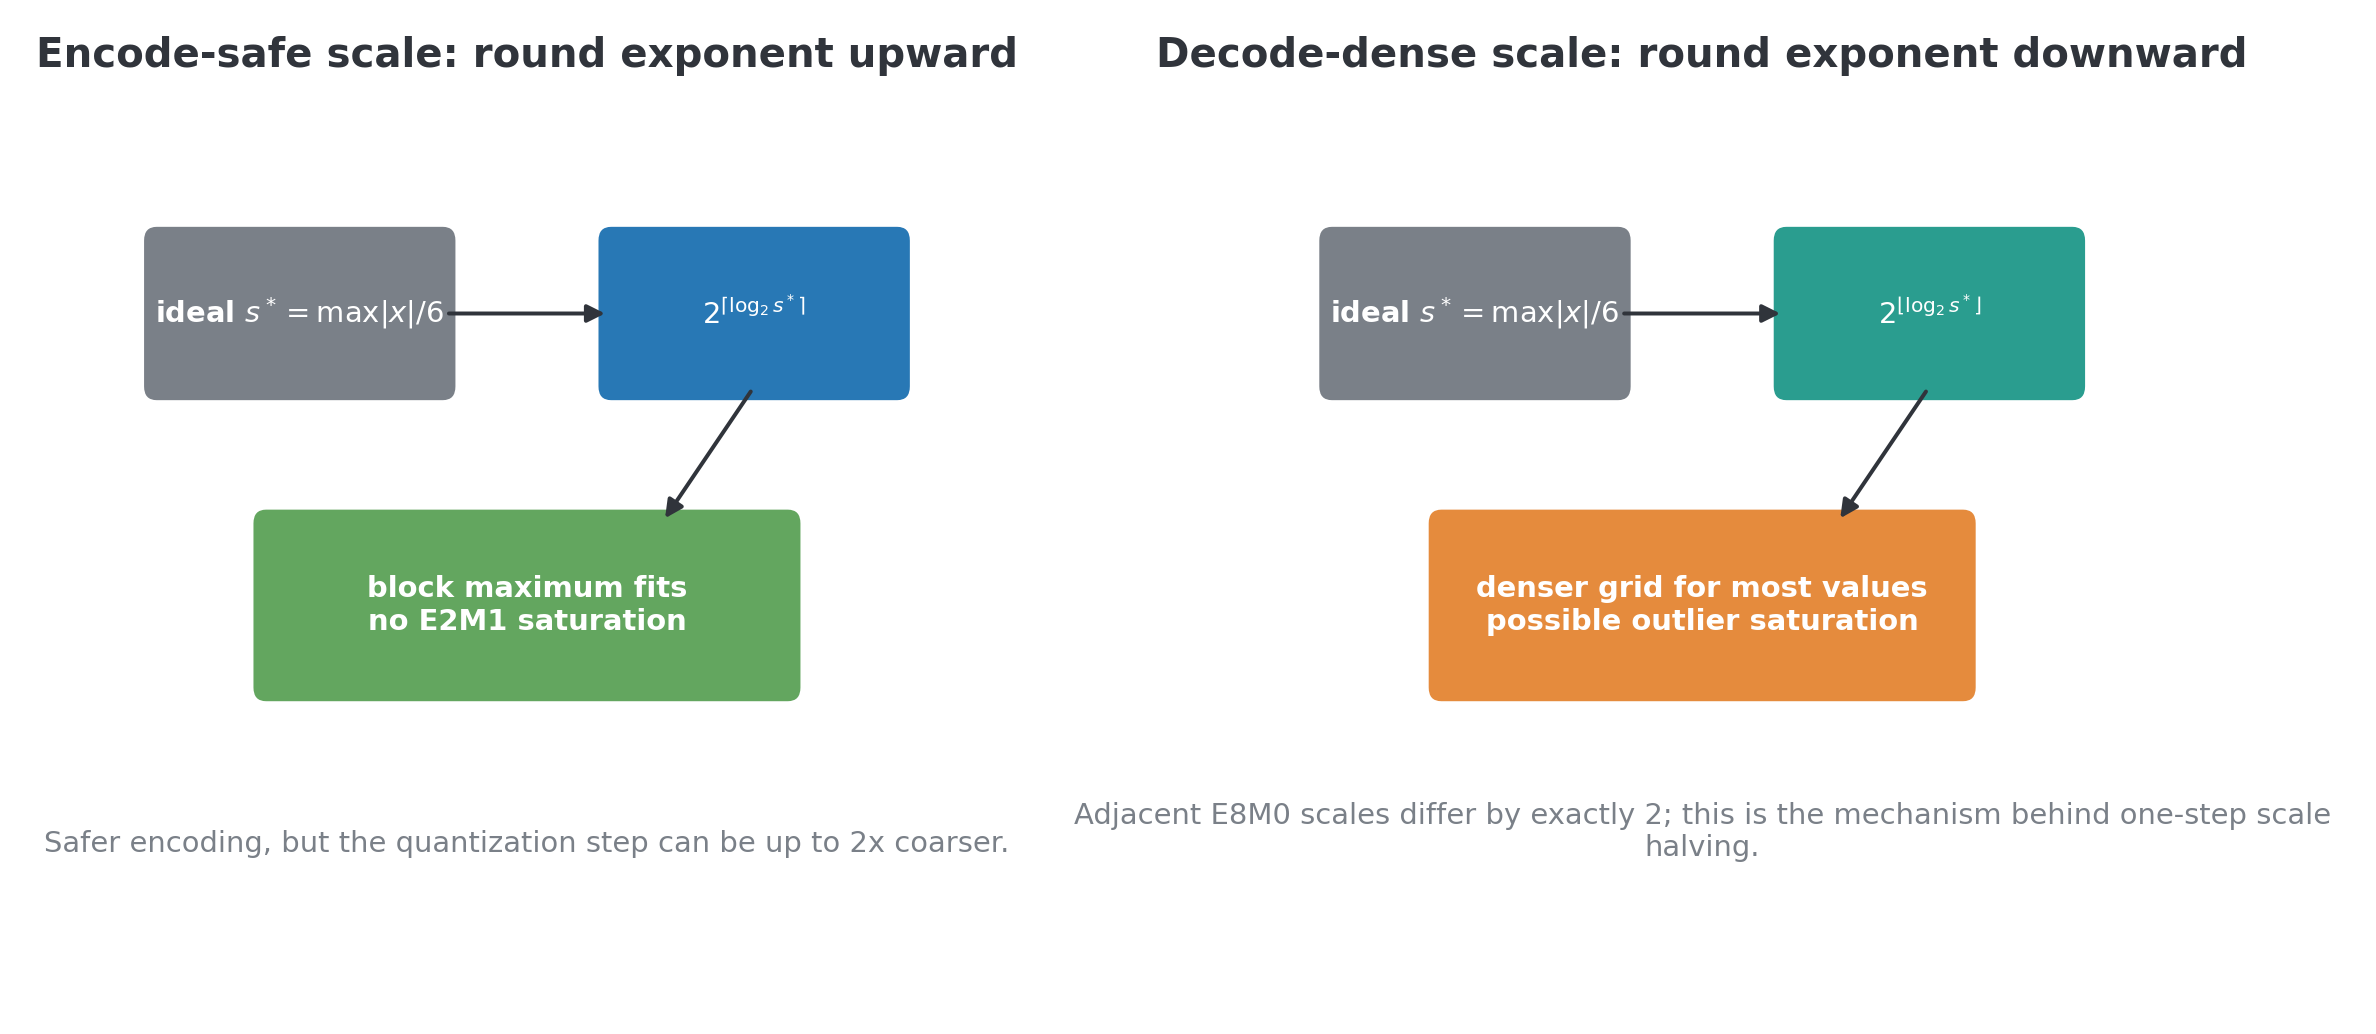
\includegraphics[width=0.96\textwidth]{figures/fp4_mxfp4_scale_rounding.png}
  \caption{Encode- and decode-centric E8M0 scale selection. Encode-centric
  scaling rounds the block maximum upward and keeps every input within the
  E2M1 endpoint. For a non-power-of-two maximum, decode-centric scaling rounds
  downward, halves the decoded grid spacing, and clips the block tail. The
  reported activation and gradient paths use the encode-centric rule. The
  2D32 weight path selects the smaller scale only under the fixed
  $a_T/s_T<0.87$ condition.}
  \label{fig:mxfp4-scale-rounding}
\end{figure}

Global \nvfp{} instead uses an E4M3 scale for
each 16 values and an FP32 tensor scale $S$ \cite{ocp2023mx,nvidia2025nvfp4}.
Its local grid is finer, but every block depends on the completed tensor amax,
the maximum absolute value.
Our global-v5 path preserves that numerical contract while replacing generic
quantize--layout--GEMM boundaries with native producers and consumers. Here,
``v5'' names an implementation generation; it is not a different NVFP4
datatype.

The CTA-local route changes only the outer-scale domain. CTA denotes the
cooperative thread array that owns a tile. For one GEMM output tile, an A-row
tile owns $\alpha_i$ and a B-column tile owns $\beta_j$.
Both remain fixed over the complete K reduction.  If $\widetilde A$ and
$\widetilde B$ denote E2M1 values decoded with their E4M3 per-block scales,
often called microscales, then
\begin{equation}
  C_{ij}=\alpha_i\beta_j
  \sum_k \widetilde A_{ik}\widetilde B_{kj}.
  \label{eq:localcta}
\end{equation}
The Tensor Core accumulates the inner sum and the epilogue applies
$\alpha_i\beta_j$ once.  This factorization is valid only because the two
outer scales are invariant in $K$, the contraction dimension. Keeping both corrections in FP32 metadata
also avoids quantizing those corrections onto the coarser FP8 scale grid.

\begin{figure}[tbp]
  \centering
  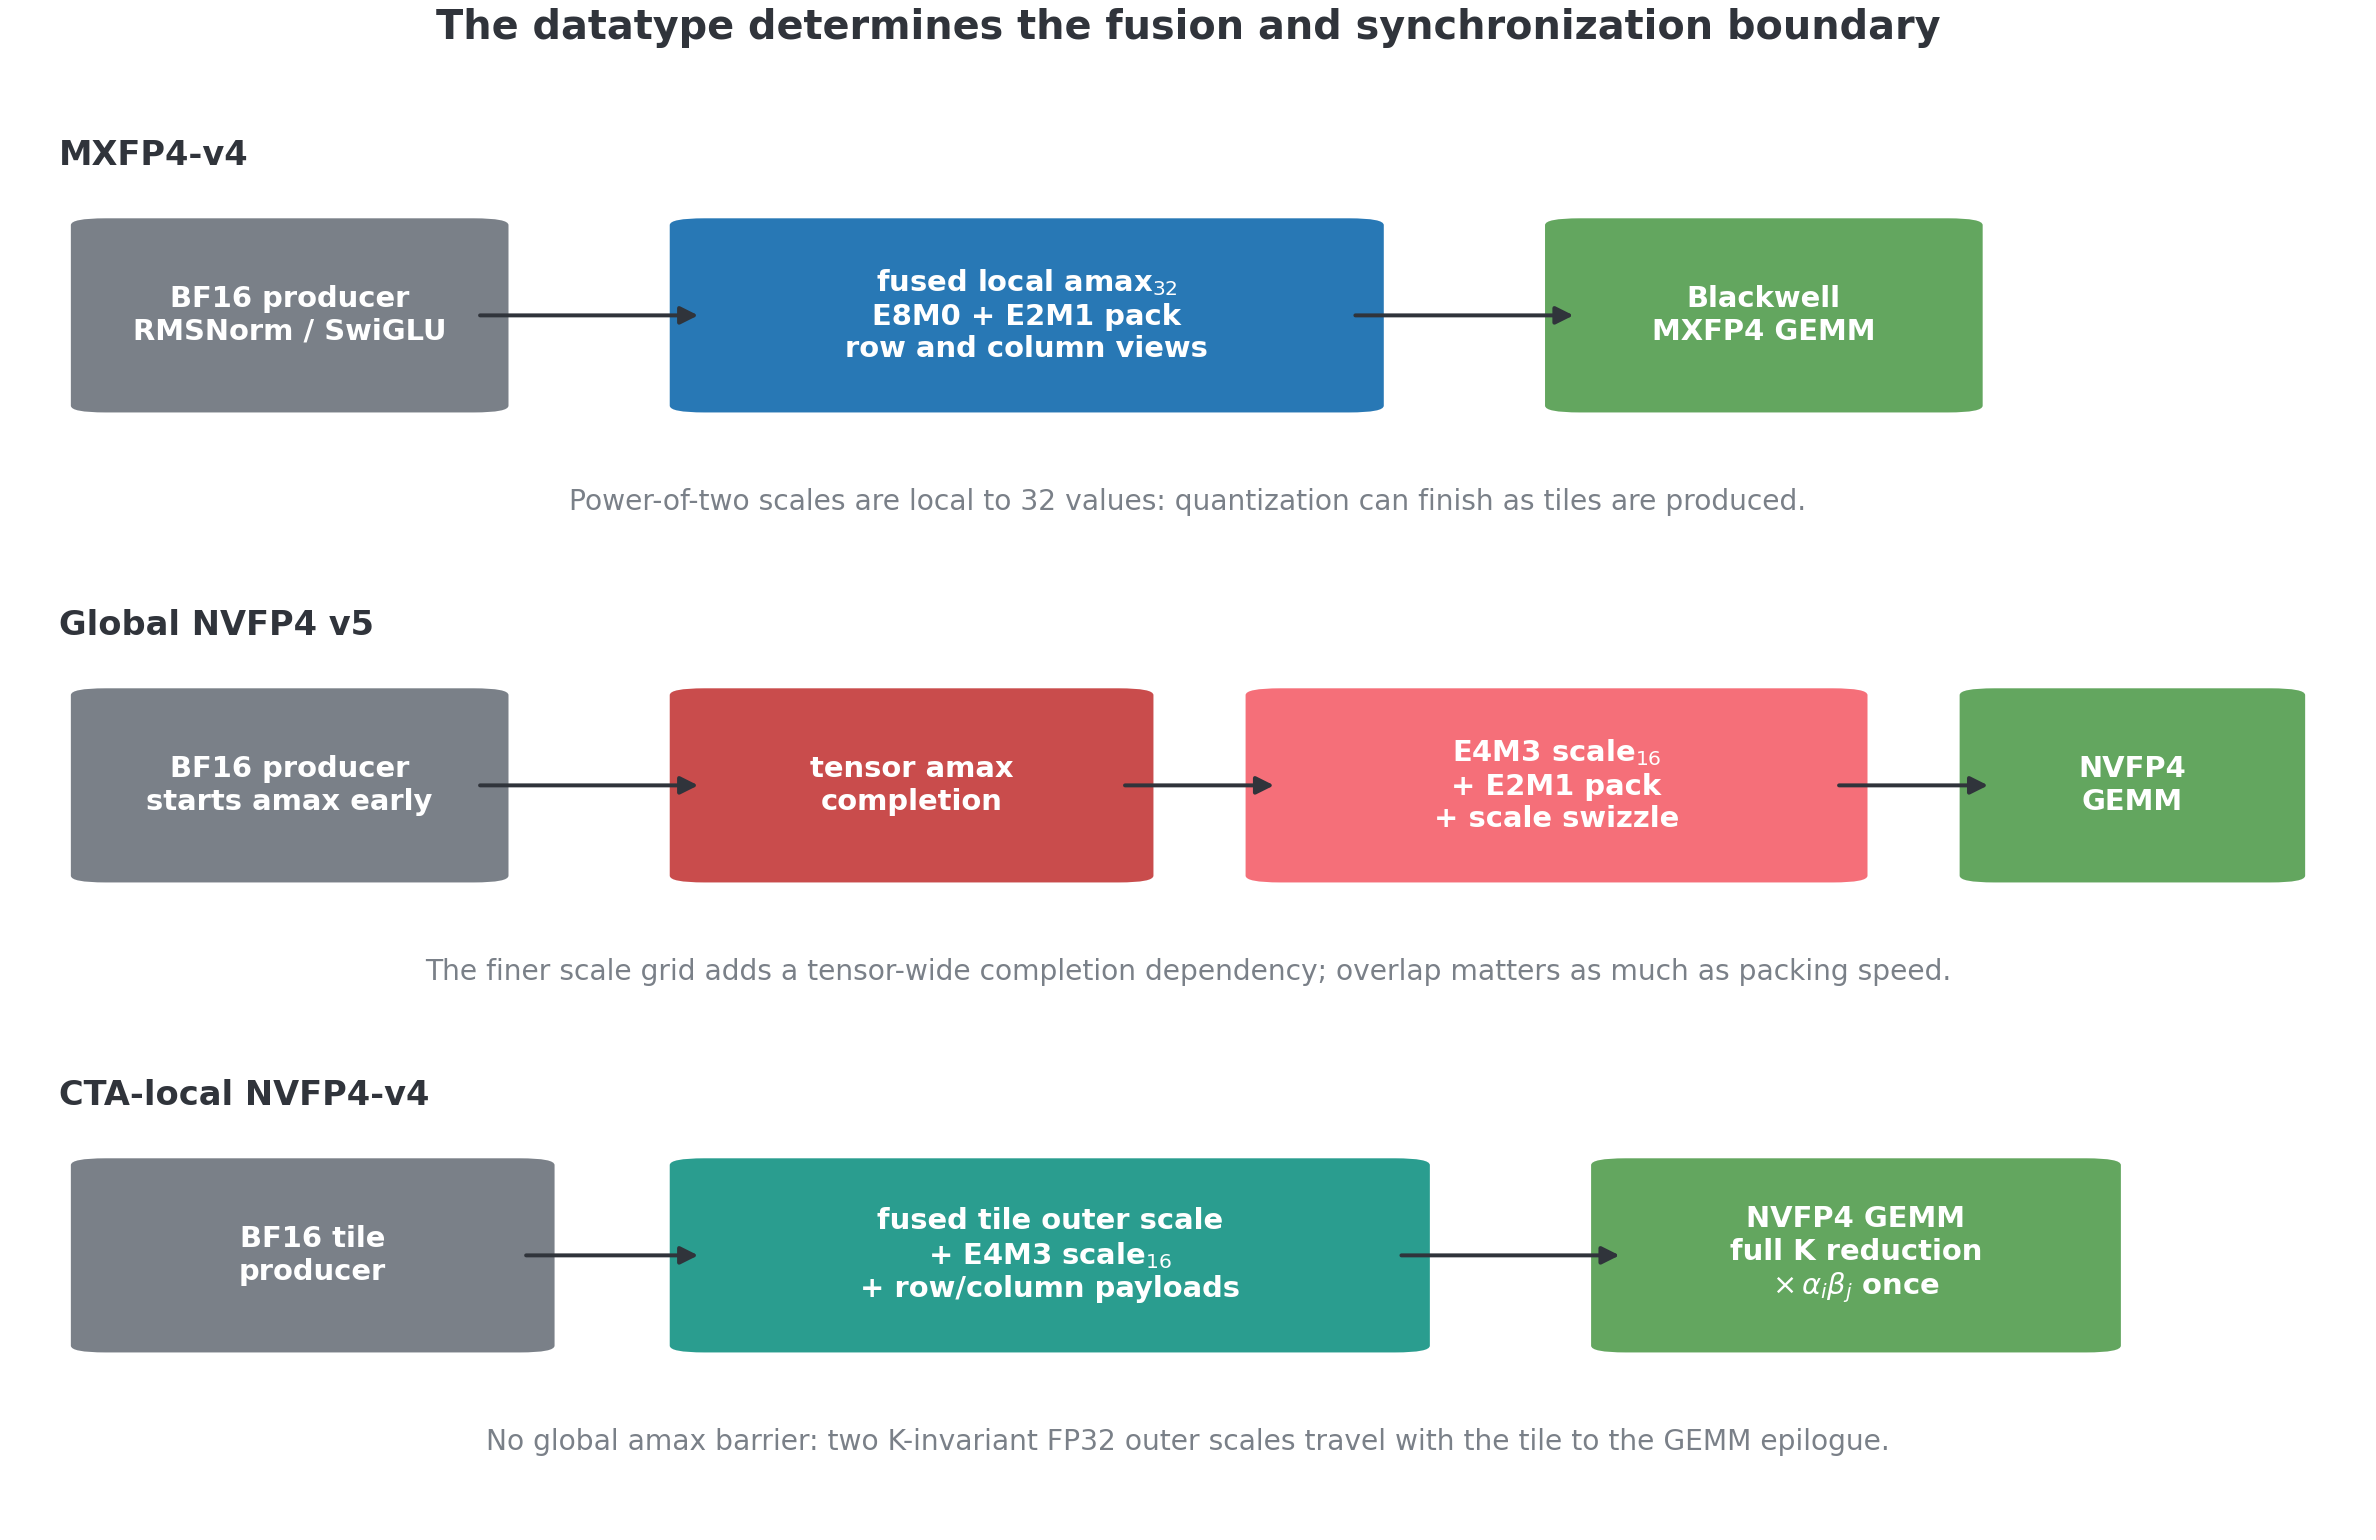
\includegraphics[width=0.98\textwidth]{figures/fp4_format_execution_routes.png}
  \caption{The formats share E2M1 payloads but expose different completion
  dependencies.  Consequently, the profitable fusion boundary is
  format-specific rather than a single generic ``FP4 linear'' kernel.}
  \label{fig:format-execution-routes}
\end{figure}

\begin{figure}[tbp]
  \centering
  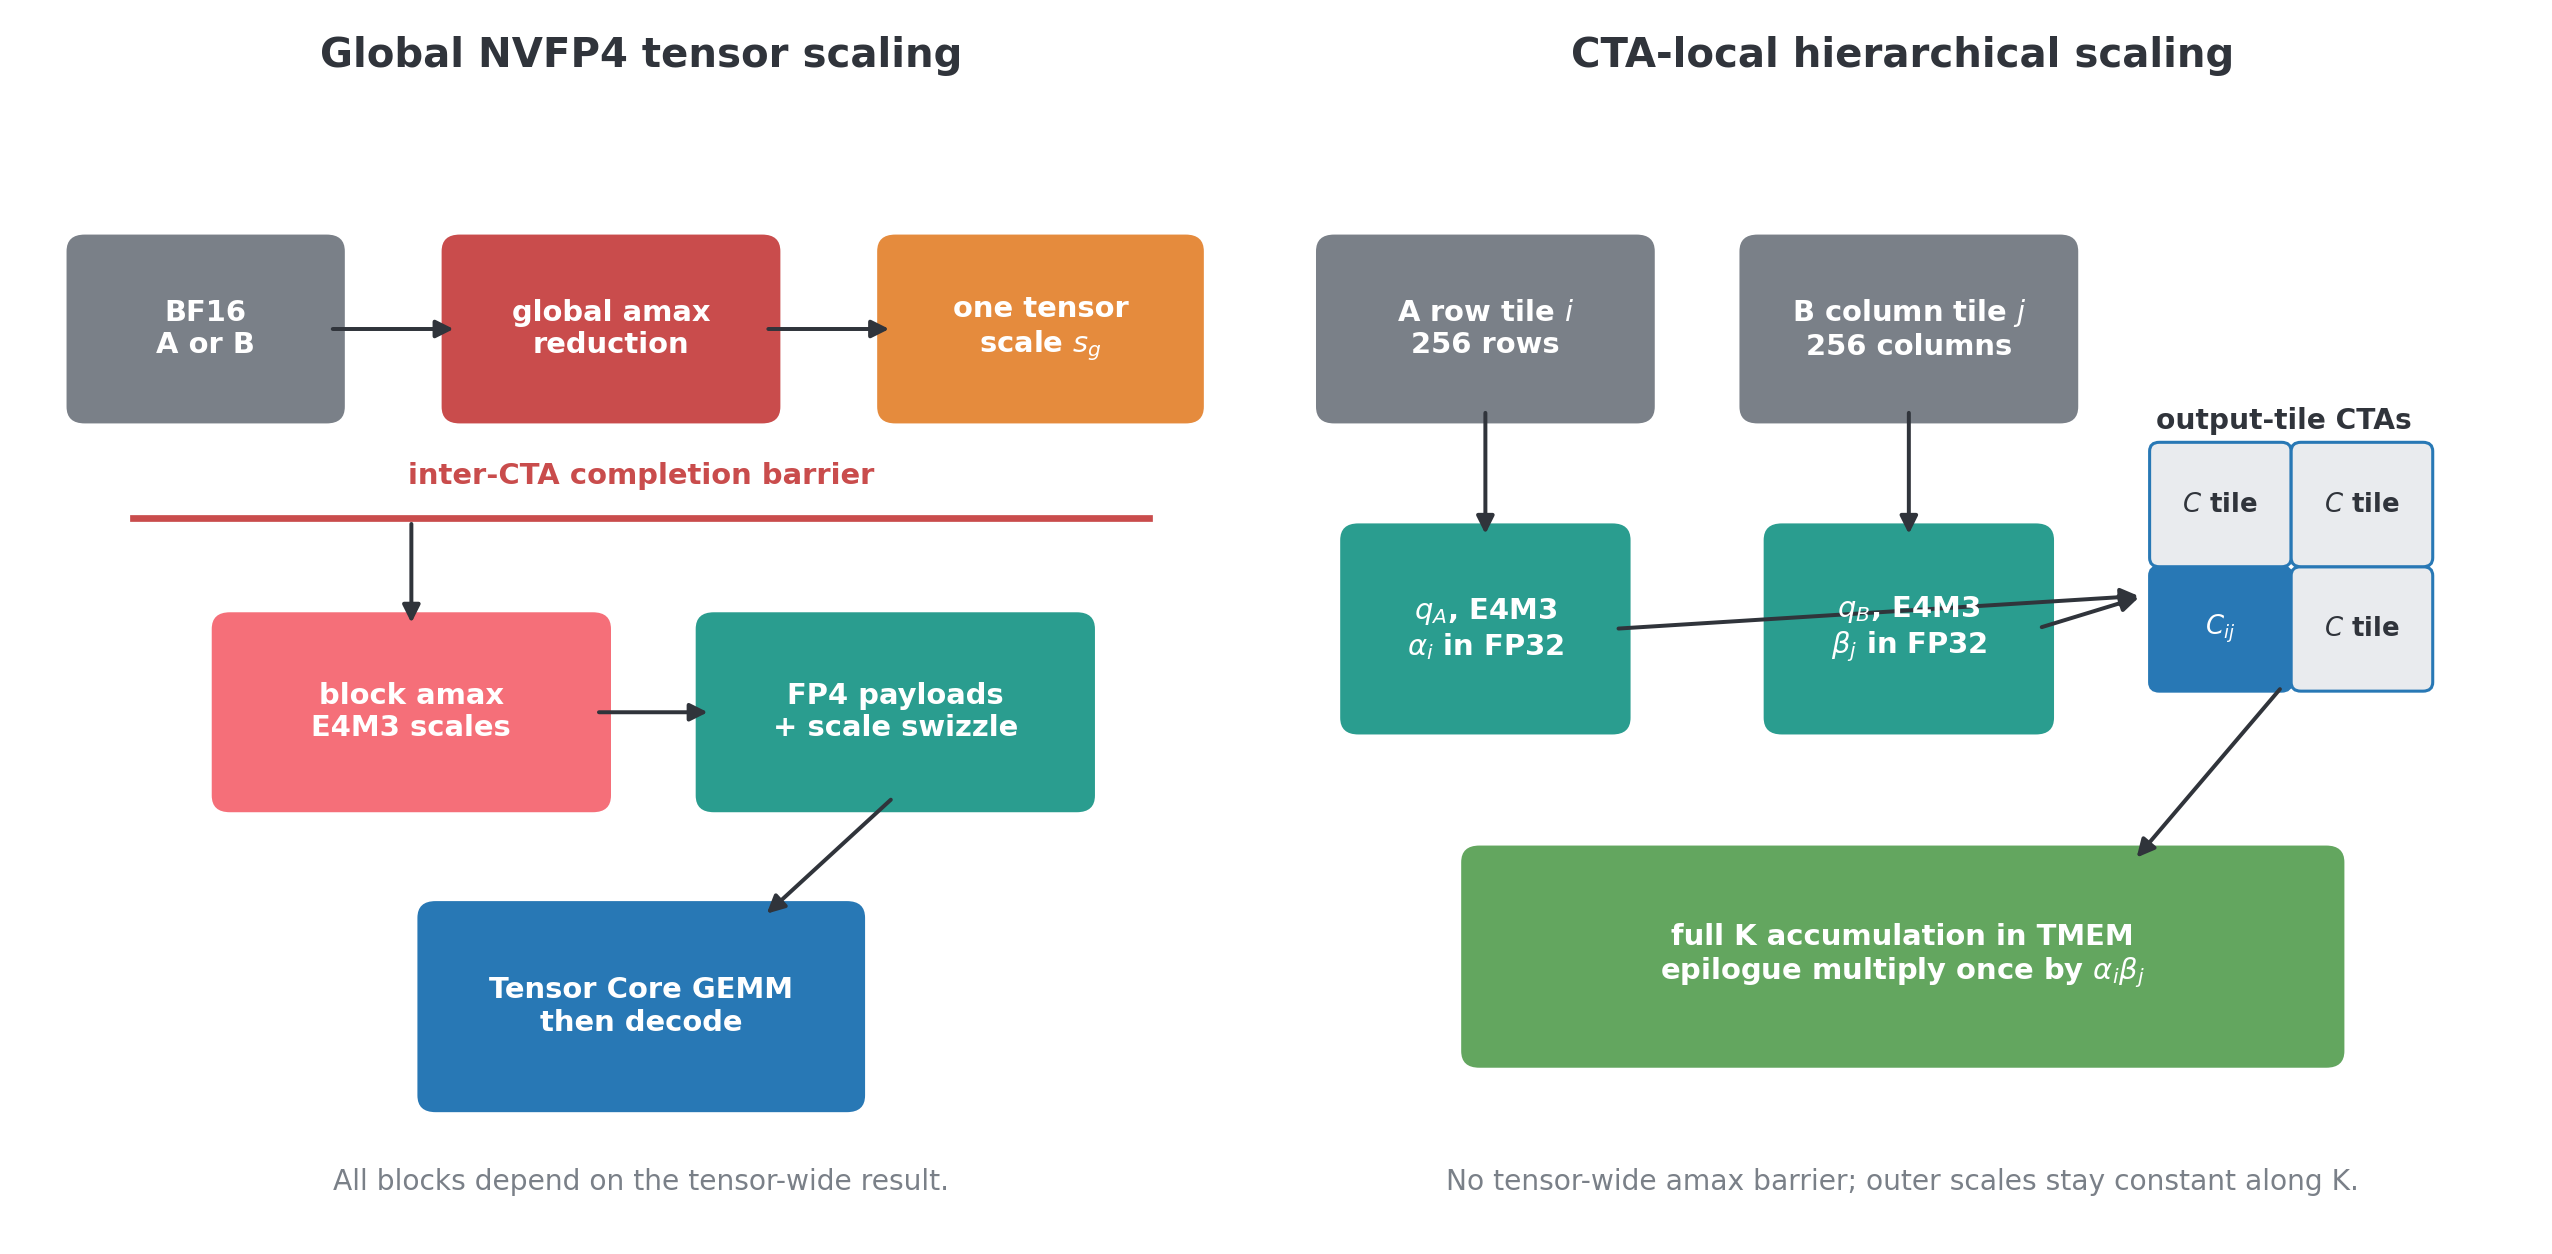
\includegraphics[width=0.94\textwidth]{figures/fp4_localcta_scaling.png}
  \caption{Global and CTA-local hierarchical \nvfp{} scaling. Global NVFP4
  completes a tensor-wide amax before finalizing its payload. CTA-local
  scaling carries row and column outer scales into the consuming GEMM and
  applies their product after the full K accumulation.}
  \label{fig:localcta-scaling}
\end{figure}

\subsection{Why forward, data gradient, and weight gradient need different views}

For a linear layer $Y=XW^{\mathsf T}$, forward propagation (Fprop), the input
or data gradient (Dgrad), and the weight gradient (Wgrad) consume different
views of the same tensors. Let $Q_r$ denote a row-facing representation and
$Q_c$ a column-facing representation. Both preserve the logical tensor shape;
the subscript identifies the physical layout and scale orientation used by the
consumer. Suppressing decode and scale metadata, training evaluates three
contractions:
\begin{align}
  \widehat Y  &= Q_r(X)Q_r(W)^{\mathsf T},
    &&\text{Fprop}, \label{eq:fprop}\\
  \widehat{dX} &= Q_r(dY)Q_c(W),
    &&\text{Dgrad}, \label{eq:dgrad}\\
  \widehat{dW} &= Q_c(dY)^{\mathsf T}Q_c(X),
    &&\text{Wgrad}. \label{eq:wgrad}
\end{align}
Thus one saved gradient needs a row-oriented payload for Dgrad and a
column-oriented payload for Wgrad; weights likewise participate in two
orientations. ``Quantize the tensor to FP4'' is incomplete unless it also
states which contraction consumes it.

\begin{figure}[tbp]
  \centering
  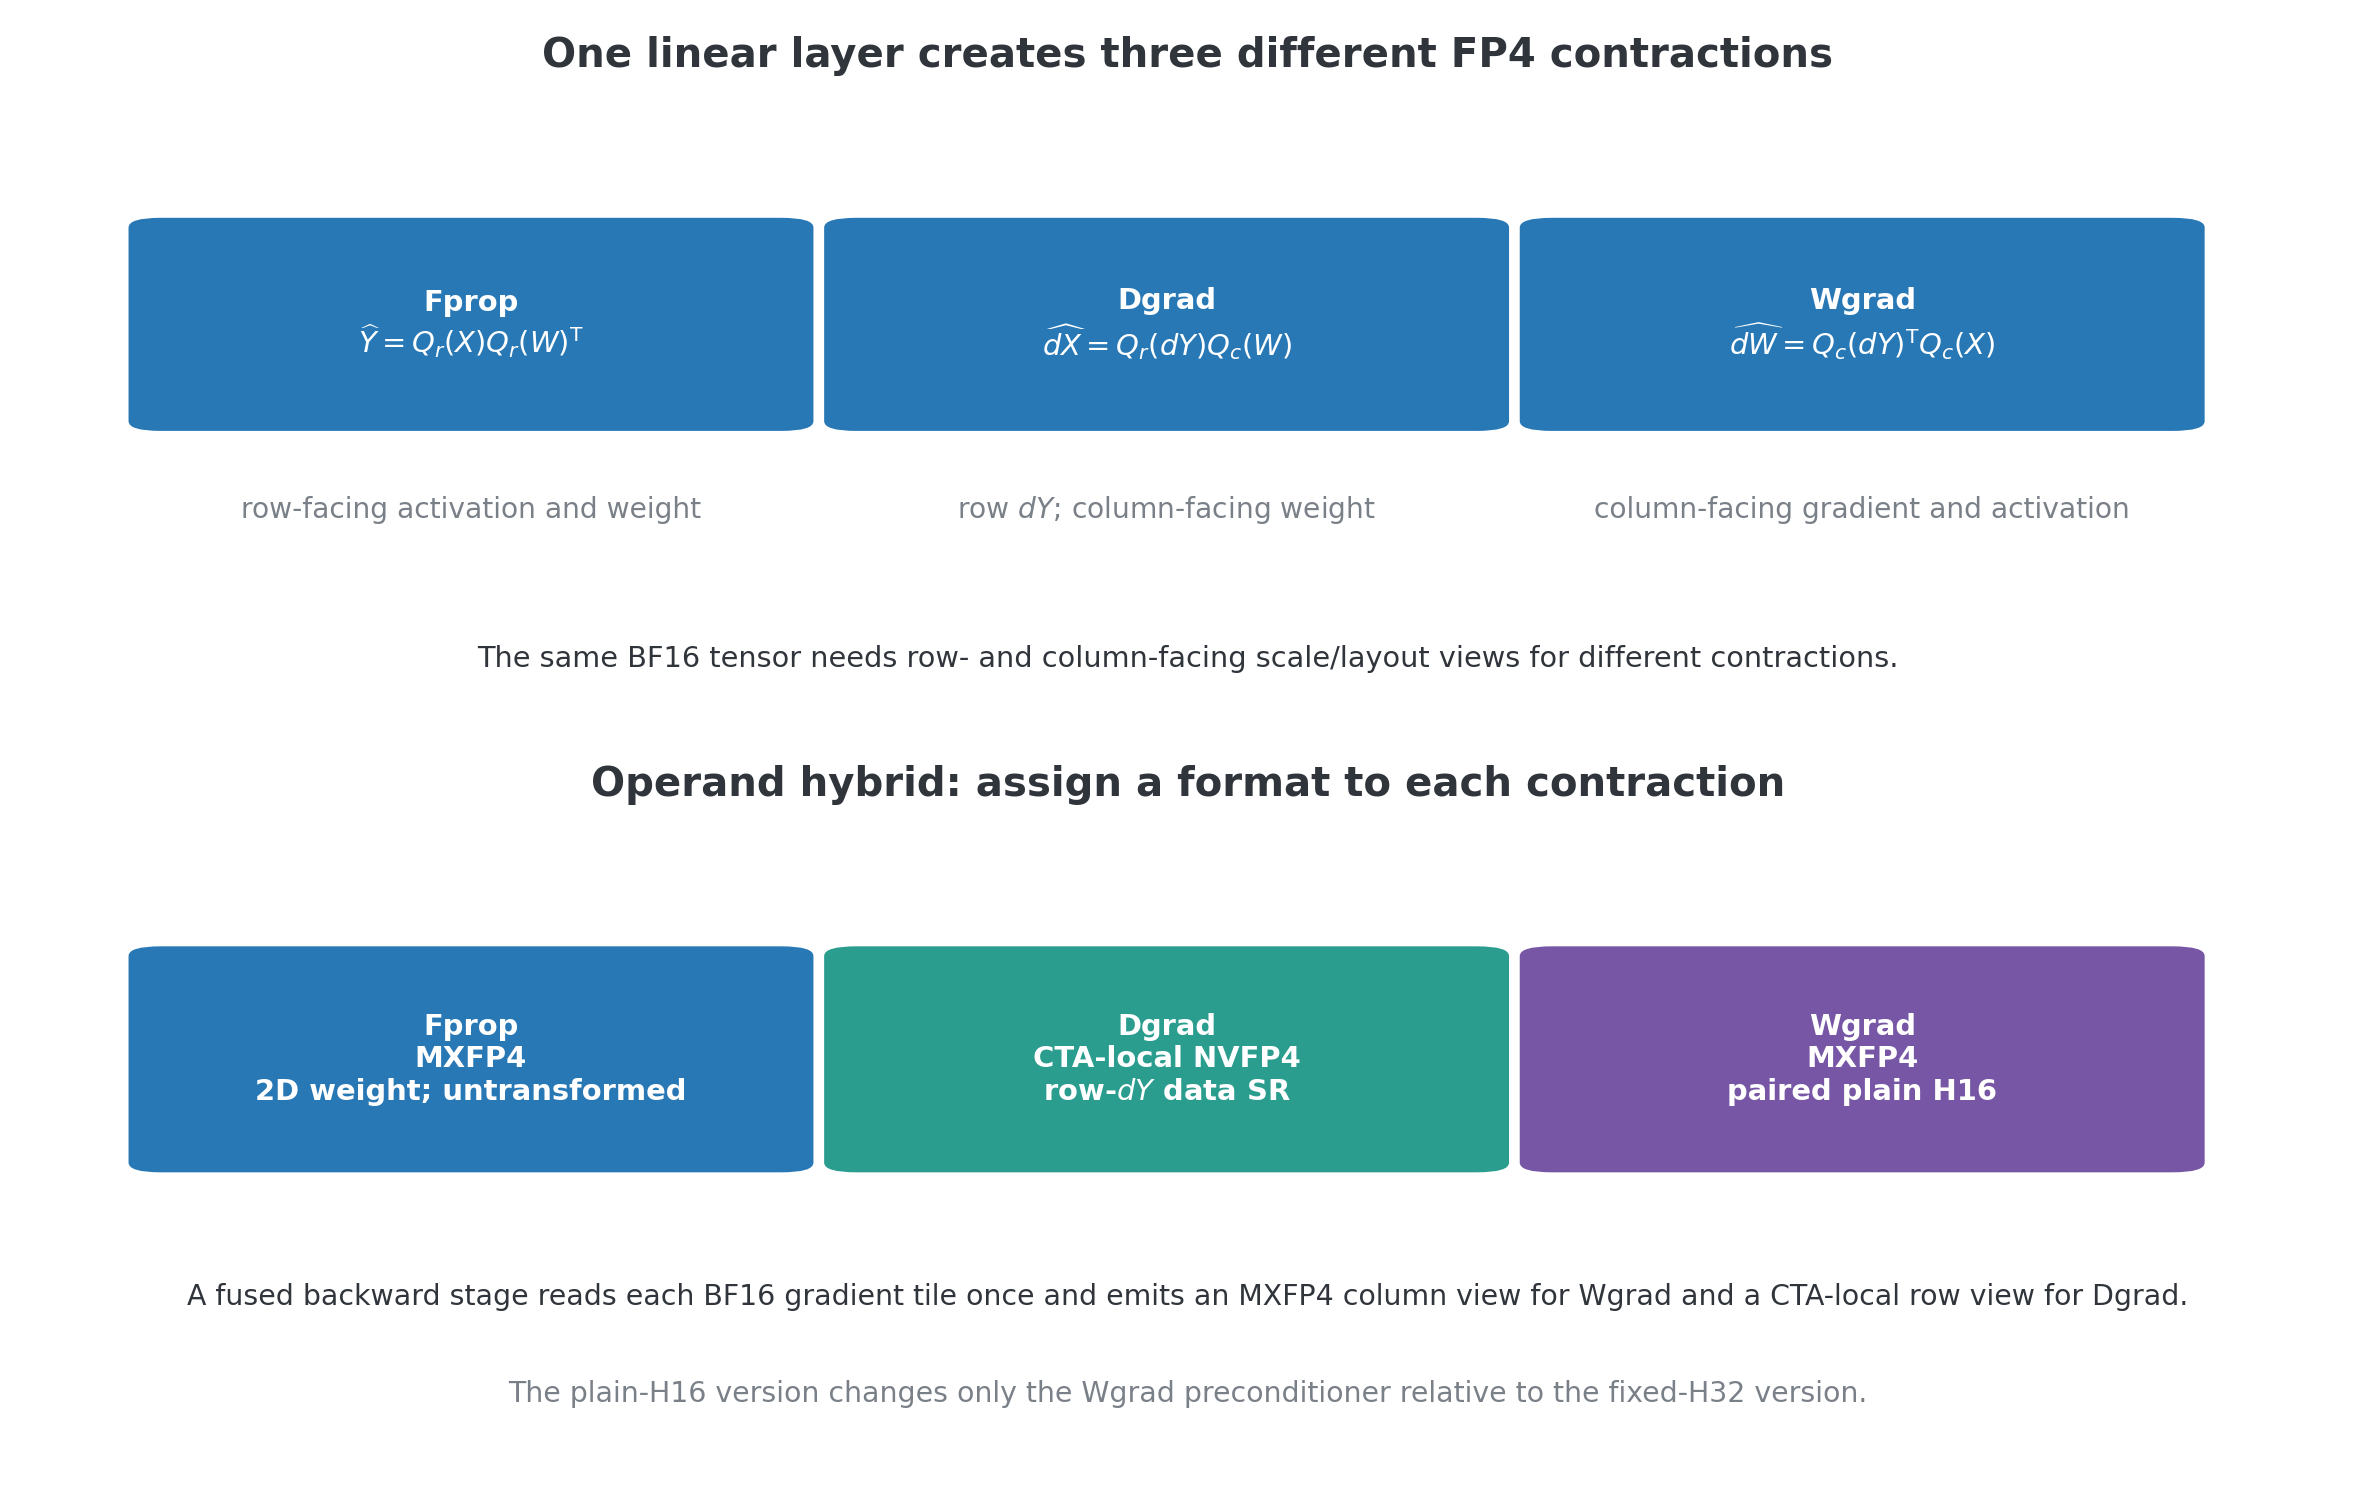
\includegraphics[width=0.97\textwidth]{figures/fp4_linear_operand_hybrid.png}
  \caption{Operand contracts for a linear layer and for the plain-H16
  operand-wise hybrid. ``Plain H16'' means a block-16 Hadamard with $D=I$ and
  no sign flips. The hybrid changes Dgrad inside every linear layer;
  it is distinct from the earlier experiment that assigned whole transformer
  blocks to different formats.}
  \label{fig:linear-operand-map}
\end{figure}

\subsection{Two-dimensional weights: numerical consistency versus implementation}

Independent one-dimensional weight quantizers can produce
$W_{\mathrm{fwd}}=Q_K(W)$ for Equation~\ref{eq:fprop} and a different
$W_{\mathrm{bwd}}=Q_N(W)$ for Equation~\ref{eq:dgrad}. Forward and backward
then consume different numerical approximations of the same BF16 weight.
Two-dimensional weight quantization instead assigns one scale to each
$b\times b$ weight tile. Let $q_{\max}$ be the largest finite E2M1 magnitude
and let $\operatorname{scale}_{\cal S}$ denote the route's scale-selection
rule on its representable scale set $\cal S$. Then
\begin{equation}
  a_{pq}=\max_{i\in p,j\in q}|W_{ij}|, \qquad
  s_{pq}=\operatorname{scale}_{\cal S}
  \!\left(\frac{a_{pq}}{S q_{\max}}\right), \qquad
  \widehat W_{ij}=S\,s_{pq}
  Q_{\mathrm{E2M1}}\!\left(\frac{W_{ij}}{S\,s_{pq}}\right),
  \label{eq:2d-weight}
\end{equation}
and reuses that numerical encoding in both orientations. The row and column
layouts can differ in memory, but their decoded weight values agree. This is
the consistency motivation identified by NVIDIA and by work on
transposition-invariant block quantization
\cite{nvidia2025nvfp4,rahimifar2026transposition}.
Equivalently, the numerical invariant is
\begin{equation}
  Q_r^{\mathrm{2D}}(W)\equiv Q_c^{\mathrm{2D}}(W)\equiv\widetilde W,
  \label{eq:2d-weight-invariant}
\end{equation}
even though the two consumer descriptors have different byte layouts.

\begin{figure}[tbp]
  \centering
  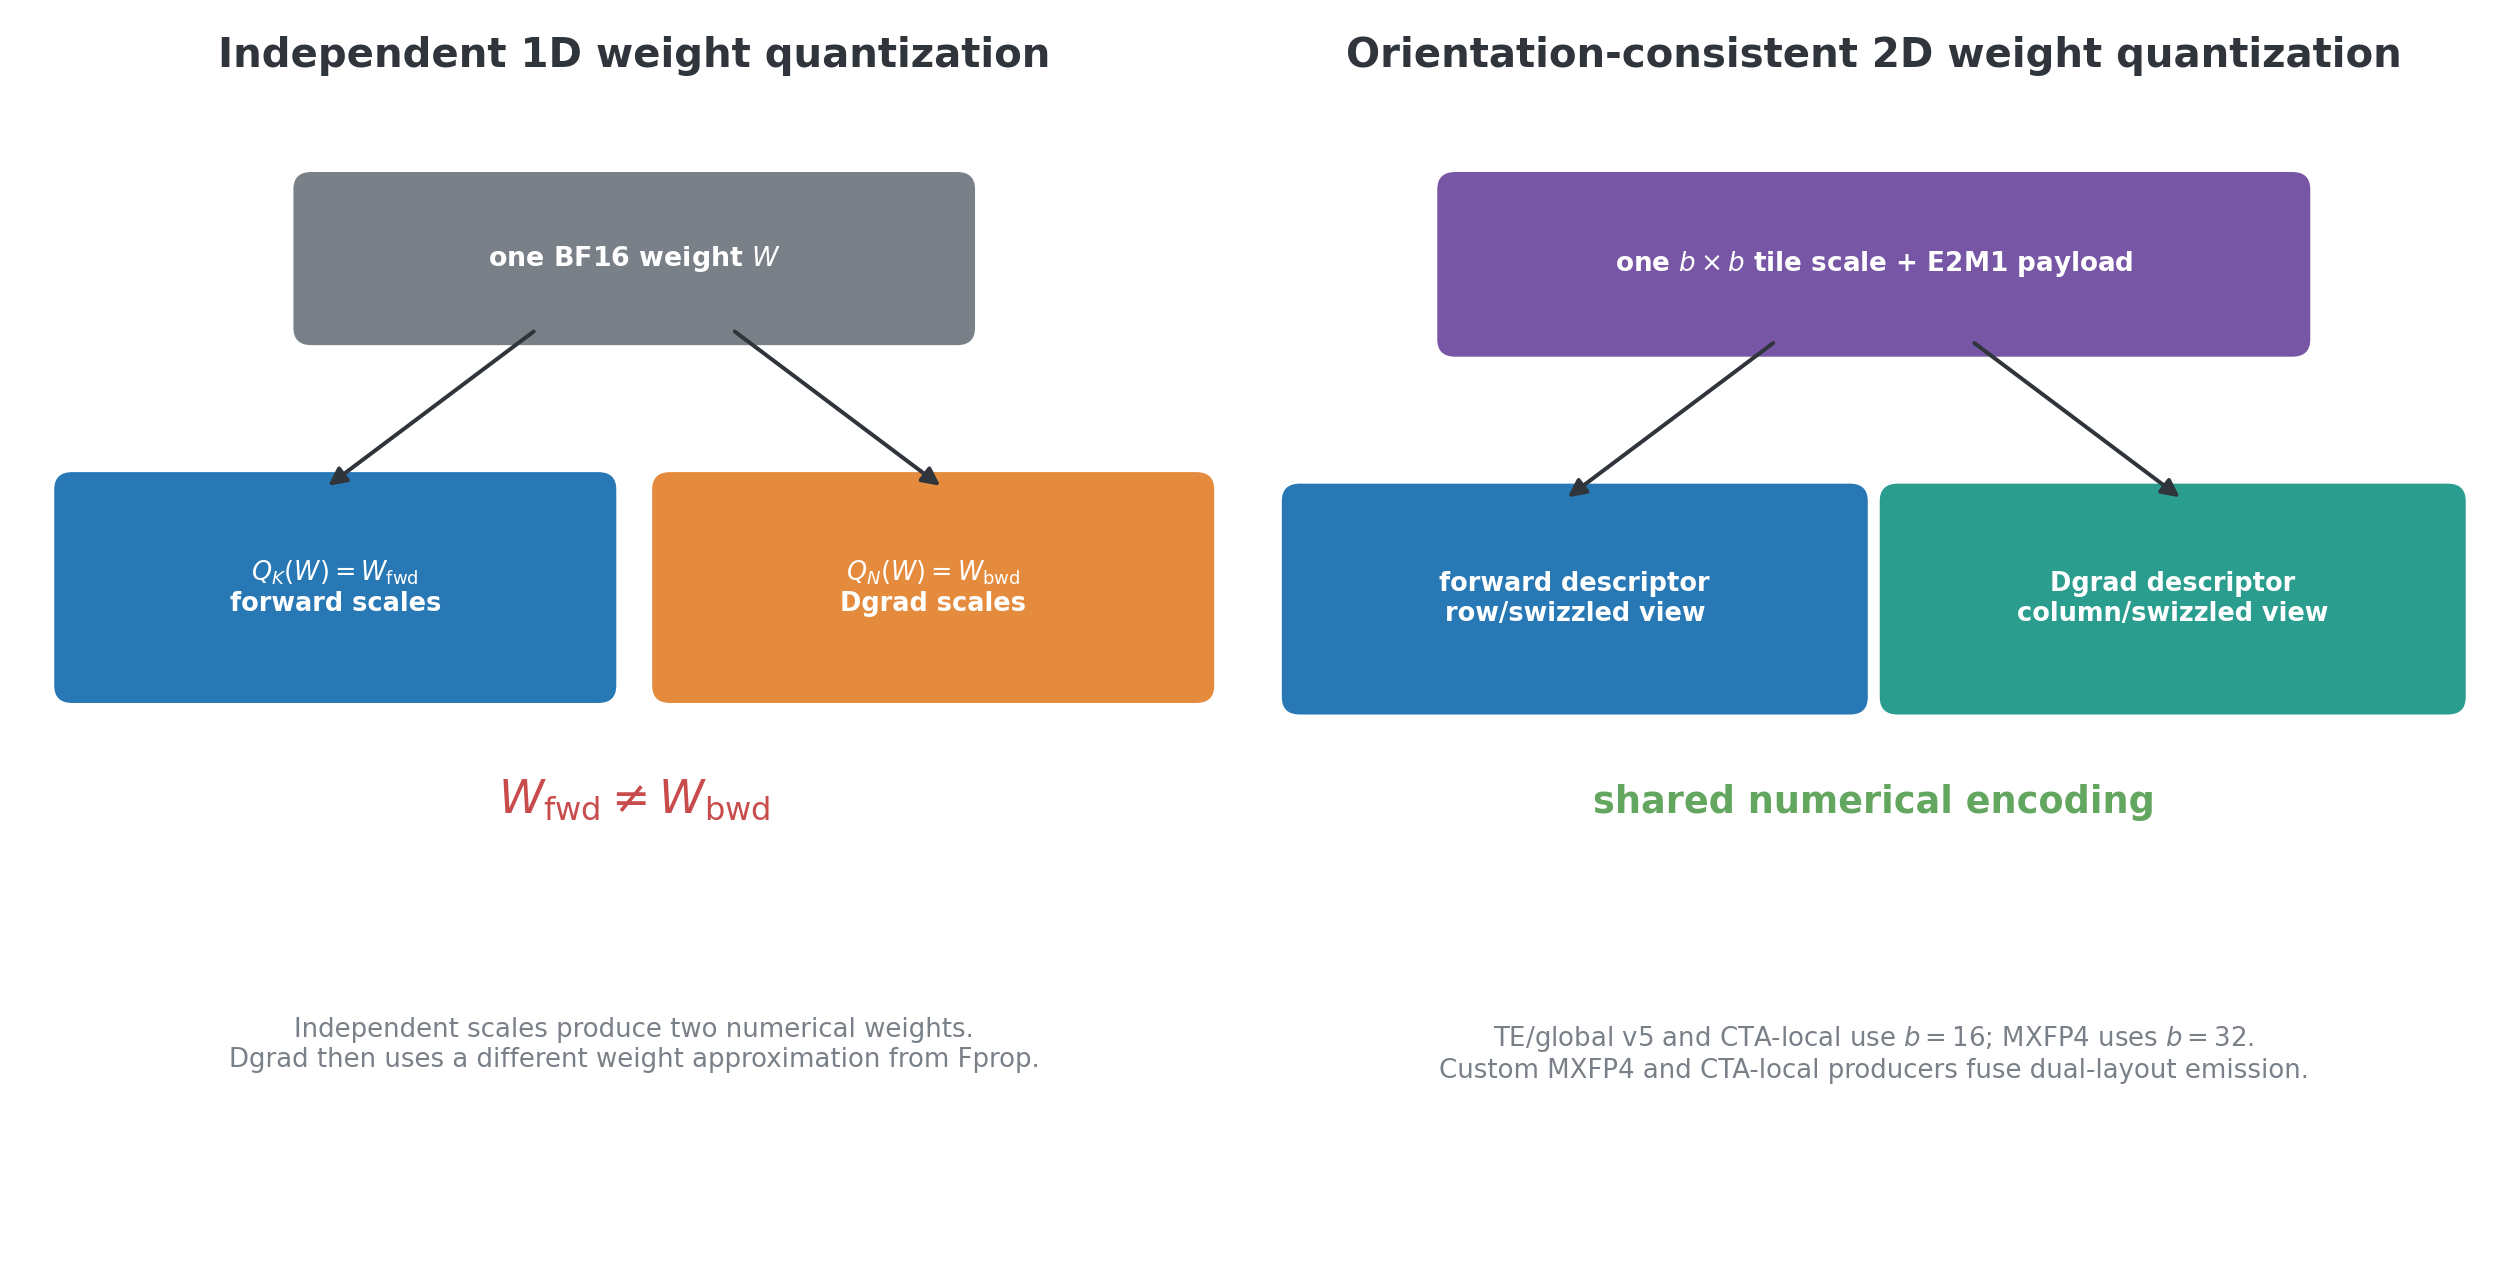
\includegraphics[width=0.96\textwidth]{figures/fp4_2d_weight_contract.png}
  \caption{One-dimensional quantization can make forward and backward see
  different weights.  A 2D tile owns one numerical encoding and exposes two
  consumer layouts.}
  \label{fig:2d-weight-contract}
\end{figure}

Transformer Engine (TE), global v5, and the CTA-local path all preserve one
numerical weight encoding across the two $16\times16$ consumer orientations.
In TE's 2D16 contract, one scale belongs to each $16\times16$ weight tile and
is replicated into the $1\times16$ scale descriptors required by the Tensor
Core consumers \cite{nvidia2025nvfp4,nvidia2026te}. ``2D'' therefore describes
shared numerical scale ownership, not a new matrix-multiplication shape. TE and
global v5 use the tensor-level NVFP4 outer scale; global v5 emits the
E2M1 values, scale metadata, and consumer layouts directly instead of
materializing TE descriptors. CTA-local NVFP4 keeps the 2D16 consistency
invariant but replaces the tensor outer scale with the tile-owned factors in
Equation~\ref{eq:localcta}. Our \mxfp{} path applies the same
orientation-consistency objective to $32\times32$ MX tiles. Tseng et al.'s
backward-only MXFP4 method instead
quantizes each operand along the reduction axis of the current contraction
\cite{tseng2025mxfp4}. Transpose-consistent 2D32 MXFP4 is prior art
\cite{cim2026nativemxfp4}; our contribution is to generate both consumer
layouts inside the fused Llama execution path.

Equation~\ref{eq:2d-weight-invariant} applies to the pure routes and the
depth-wise hybrid. The operand-wise hybrid is an explicit exception: it reads
the BF16 weight once, then emits a 2D32 MX weight encoding for Fprop and a 2D16
CTA-local weight encoding for Dgrad. Wgrad does not consume $W$; it separately
quantizes $X$ and $dY$ with MXFP4. This gives each contraction a different
error profile, so end-to-end training must evaluate the tradeoff.

\subsection{Stochastic rounding and signed Hadamard preconditioning}

For adjacent representable values $q_-$ and $q_+$, data stochastic rounding
(SR) uses
\begin{equation}
  \Pr[Q_{\mathrm{SR}}(z)=q_+]
  =\frac{z-q_-}{q_+-q_-}, \qquad
  \Pr[Q_{\mathrm{SR}}(z)=q_-]=1-\Pr[Q_{\mathrm{SR}}(z)=q_+],
  \label{eq:sr}
\end{equation}
which is unbiased between the two grid points before saturation
\cite{gupta2015limited,ozkara2025sr}. This is the ideal probability rule;
implementations that use too few random bits can introduce bias
\cite{fitzgibbon2025fewbits}. Equation~\ref{eq:sr} is ordinary adjacent-bin SR,
not LUQ. LUQ also stochastically handles values below the logarithmic FP
minimum and selects the range to avoid clipping \cite{chmiel2023accurate}. Our
microscaled E2M1 paths can saturate, so we claim removal of deterministic bias
between adjacent finite values, not unbiasedness of the complete saturated
quantizer.

The placement also differs. FP4 All the Way applies SR to the neural gradient
entering Dgrad and to both the neural-gradient and activation operands entering
Wgrad \cite{chmiel2025fp4alltheway}. NVIDIA recommends round-to-nearest for
weights and activations and SR for the gradient input to both Dgrad and Wgrad
\cite{nvidia2025nvfp4}. Our custom long routes are narrower: data SR is enabled
only on the row-oriented $dY$ representation consumed by Dgrad. The Wgrad
column representation of $dY$, weights, activations, and all scale values
remain deterministic. This axis-selective placement is a route choice evaluated
here, not a new stochastic estimator.

Hadamard preconditioning addresses a different failure mode. One outlier can
set the scale for a whole block, leaving fewer useful E2M1 values for the other
entries. A Hadamard transform mixes the block with additions and subtractions
before quantization, spreading a large coordinate over the block. In Wgrad,
this can keep smaller contributions from underflowing to zero. The transform
must be applied to both inputs of the weight-gradient dot product so that it
cancels in exact arithmetic
\cite{ashkboos2024quarot,tseng2025mxfp4,nvidia2025nvfp4}. If $H$ is the
normalized block Hadamard matrix and $R=HD$ uses a sign diagonal $D$, then
\begin{equation}
  dW=dY^{\mathsf T}X=(R dY)^{\mathsf T}(R X),
  \qquad R^{\mathsf T}R=I.
  \label{eq:paired-rht}
\end{equation}
Both Wgrad operands must therefore be transformed as a pair. Transforming only
$dY$ changes the gradient rather than only changing its quantization basis.

The Hadamard matrix itself is deterministic. In a randomized Hadamard
transform (RHT), ``randomized'' refers to how the signs in $D$ are selected;
it does not require a new sign draw at every optimizer step. Tseng et al.
sample signs and transform both MXFP4 backward GEMMs:
$(dY,W)$ for Dgrad and $(dY,X)$ for Wgrad, using a 64-value transform in their
main experiments \cite{tseng2025mxfp4}. NVIDIA's NVFP4 recipe instead
transforms Wgrad only, using a 16-value Hadamard (H16) for NVFP4 and a 32-value
Hadamard (H32) for its MXFP4 comparison
\cite{nvidia2025nvfp4,nvidia2026te}. NVIDIA samples one sign vector and shares
it across linear layers and training steps; it is fixed during the run but
random at setup \cite{nvidia2025nvfp4}. H16 and H32 name the number of values
mixed by the transform.

Our custom kernels instead specify one sign diagonal as part of the route. H16
uses a fixed 16-entry pattern, and H32 repeats that motif over two 16-value
halves. No sign vector is sampled at setup or during training. We therefore
call these paths \emph{fixed-sign H16/H32
preconditioning}, rather than RHT. The additions and subtractions mix
the values; the fixed signs choose which values are negated first. Applying
the same transform to $X$ and $dY$ preserves the unquantized Wgrad dot product,
and the stored weight is never transformed. A fixed $D$ remains orthogonal and
repeatable across layers, steps, and resumes. It does not, however, inherit a
probabilistic concentration guarantee that assumes $D$ is sampled independently
of its input. We neither claim that guarantee nor compare alternative sign
vectors.

Our recipe combines row-oriented SR only for Dgrad with paired fixed-sign
Hadamard preconditioning only for Wgrad. H16 matches the 16-value NVFP4 scale
block, while H32 matches the 32-value MXFP4 scale block. Deterministic Hadamard
preconditioning and transpose-consistent 2D32 MXFP4 have prior art
\cite{cim2026nativemxfp4}; the contributions here are their integration with
axis-selective SR, CTA-local two-sided scaling, and fused producer paths. The
literal sign pattern and its half-block construction are recorded in
Appendix~\ref{app:implementation}. Table~\ref{tab:recipe-state-ledger} states
the sign and rounding policy for every route.

\subsection{Reference NVFP4 recipe versus the routes evaluated here}

The NVIDIA recipe is a bundle, not only the NVFP4 datatype. It recommends
2D16 weights, SR on gradient inputs to Dgrad and Wgrad, a paired H16 signed
Hadamard transform (described as RHT) for
Wgrad, and retaining roughly 15\% of empirically sensitive linears in higher
precision, with most selected linears near the end of the network
\cite{nvidia2025nvfp4}. Three distinctions matter in this report. First, our
TE-native comparator enables TE's 2D, gradient-SR, and signed-Hadamard
mechanisms but places all 32 body blocks in NVFP4; only the common output head
is BF16. Second, the TE comparator with four final BF16 blocks is a separate
NVIDIA-inspired route. It is not a reproduction of NVIDIA's per-linear
sensitivity list. Third, the custom v5, \mxfp{}, and \localcta{} long routes
use row-Dgrad SR, and only explicitly named routes apply Hadamard
preconditioning. Tables~\ref{tab:recipe-ledger}
and~\ref{tab:recipe-state-ledger} state the complete contract for each result.
\FloatBarrier
